\chapter{Algoritmos e Fluxograma}
\section*{Introdução}
    \paragraph{}
    Neste capítulo veremos o que significa algoritmo, o que é uma tela LCD e para que ela serve. Além disso, vamos abordar o conceito de linguagem de programação e saber, afinal, como nos comunicar com o \textit{Sparki}. E aí, vamos nessa?
\section{Algoritmo e Diagrama de Fluxos}
    \paragraph{}
    Diariamente utilizamos algoritmos sem mesmo perceber. Quando cozinhamos um macarrão, assamos um bolo, montamos um móvel, um brinquedo ou mesmo quando escovamos os dentes estamos utilizando este conceito para completar essas tarefas. \par
    Isto porque tomamos essas decisões nos baseando em instruções claras para chegar a um objetivo. Então, se estamos preparando um bolo, não podemos simplesmente colocar os ingredientes no forno sem antes misturá-los conforme a receita. Não teríamos um bolo, mas sim um Frankestein! Da mesma forma, não poderíamos esperar que ele fique pronto se ligarmos o forno, mas não colocássemos a massa do bolo nele. \par
    \begin{center}
    \textbf{Definição} \\
    Algoritmo é um conjunto finito de instruções sequenciais lógicas, bem definidas, não ambíguas que levam à solução de um problema.
    \end{center}
    
    \textit{Mas afinal o que esse bando de palavras complicadas querem dizer? Eu não entendi foi nada.}\par
    O que elas querem dizer é, em outras palavras, que um algoritmo indica um conjunto de instruções para realizar uma tarefa qualquer, como por exemplo, fazer pipoca. Seguimos uma receita que nos diz bem direitinho o que fazer para atingir o objetivo desejado, que no caso é aquela pipoca bem quentinha e crocante no final das contas! Assim ficou mais fácil de entender, né? \par

    \textit{Ainda não to entendendo o que é algoritmo, tem como desenhar?} \par
    Claro! Voltamos ao exemplo da pipoca, a receita é:\par
    
  \begin{enumerate}   
    \item	Separe os ingredientes;
    \item	Na panela, coloque o óleo cobrindo todo o fundo da panela;
    \item	Coloque-a no fogo;
    \item	Coloque 3 grãos de milho e espere;
    \item	Quando estes grãos estourarem, adicione o restante do milho;
    \item	Volte com a panela para o fogo e aguarde o restante do milho estourar;
    \item	Tempere a pipoca a gosto.
    \end{enumerate} 
    
    Ou seja, um conjunto de regras e procedimentos lógicos que levam à solução de um problema em um número finito de etapas. Desenhando, a receita ficaria assim:\par
   
    \begin{figure}[h]
    \caption{Diagrama de Fluxos}
    \centering 
    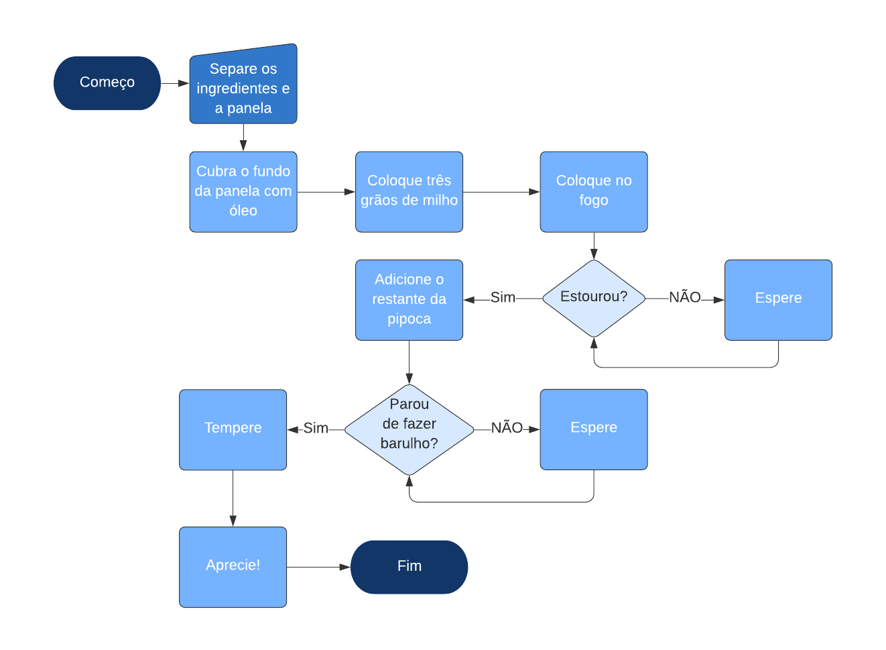
\includegraphics[width=14cm]{Figuras/Pipoca.png}
    \label{figura:Pipoca.jpeg}
    \end{figure}

    Este desenho é chamado de Fluxograma ou Diagrama de Fluxos, e nada mais é uma representação esquemática de um processo ou algoritmo. Nele são utilizadas formas geométricas para desenhar a sequência lógica de um programa, tornando-a mais fácil de ser entendida e documentada.\par
    
    \begin{center}
    \textbf{Definição} 
    \\
    Uma representação gráfica de passos sequenciais e decisões a serem tomadas durante a execução de um processo.
    \end{center}
    
    \textit{Mas por que você desenhou apenas com quadrados ou círculos ao invés de usar todas formas diferentes?}\par
    Para facilitar o entendimento e a comunicação com outros programadores, costumamos seguir um padrão, dessa maneira temos as seguintes figuras descritas na figura \ref{figura:formas.jpeg}.
    
    \begin{figure}[h]
    \caption{Padrão de formas geométricas}
    \centering 
    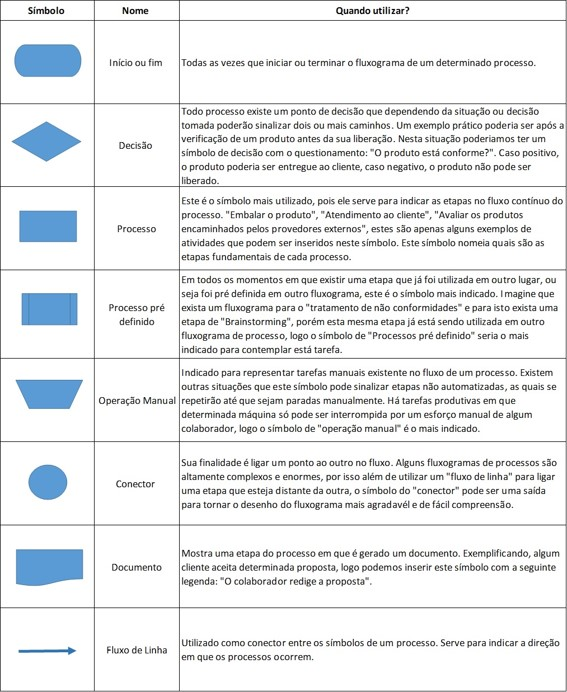
\includegraphics[width=11cm]{Figuras/formas.jpg}
    \label{figura:formas.jpeg}
    \end{figure}
     
     \paragraph{}
    Esboçar um Fluxograma antes de programar pode ser muito útil, principalmente quando se está aprendendo ainda. Dentre as principais vantagens de se fazer um Fluxograma, temos:
    \begin{itemize}
        \item Poder escolher a melhor solução para o problema;
        \item Organizar as ideias antes de começar a programar de fato;
        \item Evitar erros de lógica.
    \end{itemize}
    
    Na internet encontramos diversos sites para criar nossos diagramas, como esse da pipoca, por que você não dá uma olhada? Segue o link de algumas sugestões: \par 
    
    \begin{enumerate}   
    \item Lucidchart  - https://www.lucidchart.com/
    \item Creately - https://creately.com/ 
    \item Draw.io - https://www.draw.io/ 
    \end{enumerate}   

    Como já vimos, robôs não raciocinam como nós, seres humanos. Então, precisamos deixar bem claro o que esperamos de cada um deles quando estamos nos comunicando com eles para que o objetivo final seja cumprido.\\
    
    \textit{Ué, mas isto parece exatamente com algo que você já disse.} \par
    Exatamente! Escrevemos algoritmos para fazer a programação de robôs!\\

    Até agora vimos que algoritmos são extremamente importantes e é essencial que o seu conceito seja entendido. Mas você sabia que não precisamos de um computador para programar? 
    
\subsection{Torre de copos}
    \begin{figure}[h]
    \caption{Exemplo de um torre feita com copos}
     
    \centering 
    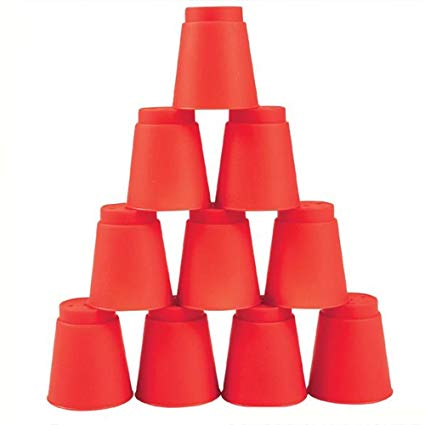
\includegraphics[width=8cm]{Figuras/torre.jpg}
    \label{figura:torre.jpeg}
    \end{figure}

\paragraph{}
Que tal vermos um exemplo de como você pode criar um algoritmo de forma fácil e prática? Tudo o que você precisa é de alguns copos (de preferência de plástico) e de algum lugar para escrever. Agora, você deve começar a criar instruções básicas e necessárias para transformar uma pilha normal de copos em uma majestosa torre de copos. Para isso utilize comandos como: "\textbf{pegar copo}", "\textbf{soltar copo}", "\textbf{mover o copo para cima, para a direita ou esquerda}" e outras que você julgar úteis, desde que todas elas sejam bem simples e diretas (sem duplo sentido). Ah, você não pode simplesmente escrever a instrução "\textbf{monta torre}" ou "\textbf{vire de cabeça para baixo}", porque você não deixou claro se é para virar o copo de cabeça para baixo, ou a pessoa de cabeça para baixo, ou a cadeira, e etc.

Agora que você tem todo o seu conjunto de instruções, hora de organizá-las de forma sequencial para que você mesmo ou o seu amigo siga elas a fino, e assim seja capaz de no final ter uma torre de copos montada em sua frente.

Exemplo: "\textbf{pegar copo, mover copo para direita, soltar copo, mover a mão para esquerda, pegar copo...}"

Como o que você acabou de fazer é um conjunto finito de instruções bem definidas sem ambiguidade, simples e escritas de forma sequencial, onde tudo foi feito com o objetivo de realizarmos uma tarefa (montar a torre), podemos concluir, então, que o que você fez \textbf{é um algoritmo}.

\section{Linguagem de programação}
    Se fosse dado o comando abaixo para o \textit{Sparki} você acha que ele entenderia? \par
    \begin{center}
    Sparki vai para frente! Sparki vai para trás!\ \par
    \end{center} \par
    Quem pensou que ele não entenderia acertou, o \textit{Sparki} não iria entender nada do que foi dito.\\
    
    \textit{Então como ele entende os comandos que pedimos para ele fazer?}\par
    Para nos comunicarmos com o \textit{Sparki}, é preciso passar os comandos para o computador através de uma linguagem de programação, que irá converter o que escrevemos para 0's e 1's e depois enviará para \textit{Sparki}, e assim ele será capaz de entender e executar o comando.
    
    \begin{center}
    \textbf{Definição} \\
    Uma linguagem de programação é um método padronizado para comunicar instruções para um computador.
    \end{center} \par
    
\paragraph{}
De maneira mais simples, linguagem de programação é a língua que usamos para nos comunicar com o computador assim como a língua portuguesa é a língua que usamos para nos comunicar entre nós. Assim como existem várias línguas como inglês, alemão e japonês, existem várias linguagens de programação cada uma com suas peculiaridades, mas aqui no nosso curso iremos focar em aprender a linguagem que o \textit{Sparki} usa.

\paragraph{}
Como mencionado anteriormente, o que escrevermos para o \textit{Sparki} é antes transformado em 0's e 1's, isso porque os computadores utilizam a notação \textbf{binária}, onde os números são representados apenas utilizando-se de 0's e 1's. Podemos concluir então que, na verdade, os computadores não entendem a linguagem de programação!! Tudo o que escrevemos para eles em linguagem de programação é depois transformado em 0's e 1's para que finalmente possamos nos comunicar.
    
 
\subsection{Funções importantes: void setup(), void loop()}
    
    \paragraph{}
    O comando \lstinline[columns=fixed]{#include <Sparki.h>} e as funções \lstinline[columns=fixed]{void setup()} e \lstinline[columns=fixed]{void loop()} são as funções mais importantes na hora de começar a programar o \textit{Sparki}, pois entender o que elas significam e como funcionam é essencial para saber onde escrever determinada parte do código em relação ao tipo de aplicação.
    
    \begin{lstlisting}[language=C]
#include <Sparki.h>;

void setup()
{
}

void loop()
{
}
\end{lstlisting}


    \begin{itemize}
        \item Biblioteca \lstinline[columns=fixed]{sparki.h}: Esta biblioteca guarda todas as funções relacionadas ao \textit{Sparki}, e é necessário inserir ela na primeira linha de código, para que estas funções sejam habilitadas para a comunicação entre o computador e o robô funcionar.
        \item \lstinline[columns=fixed]{void setup()}: Esta função é a primeira a rodar no código, e tudo que está dentro de suas chaves é executado apenas uma vez. A função é bastante útil para inserir configurações iniciais, como por exemplo limpar a tela LCD, ou fazer algum movimento inicial que não irá se repetir no resto do programa.
        \item \lstinline[columns=fixed]{void loop()}: Esta função é usada para colocar códigos que irão ficar se repetindo no programa, ou seja, sempre ficará rodando até que seja carregado algum outro programa no \textit{Sparki}. Um exemplo para esta função é deixar o \textit{Sparki} sempre com o LED de uma cor ligado, ou sempre se movimentando em uma determinada direção.
        \end{itemize}

  \section{Exercícios}

\question{Em suas palavras, defina o que é um algoritmo e dê 2 exemplos não citados no capítulo.}
    \begin{center}
    \line(1,0){450}
    \vspace{0.2cm}   
    \line(1,0){450}
    \vspace{0.2cm}   
    \line(1,0){450}
    \vspace{0.2cm}   
    \line(1,0){450}
    \vspace{0.2cm}   
    \line(1,0){450}
    \vspace{0.4cm}   
    \end{center}
    
\question{O objetivo de uma linguagem de programação é:}
    \begin{enumerate}
        \item Fornecer um conjunto de regras bem definidas que permita escrever programas de computador de forma mais amigável evitando ambiguidades.
        \item Dar a liberdade para cada programador escrever programas de computador a partir do seu próprio conjunto de regras, facilitando o processo de programação.
        \item Estabelecer regras para comunicação entre seres humanos.
        \item Definir um padrão para programadores utilizarem os comandos binários intrínsecos a cada arquitetura de processador.
    \end{enumerate}
    
\question{Considerando o labirinto abaixo elabore um fluxograma indicando o caminho que o Sparki deve seguir para encontrar a saída}
    
    \begin{figure}[h]
        \caption{labirinto}
        \centering 
        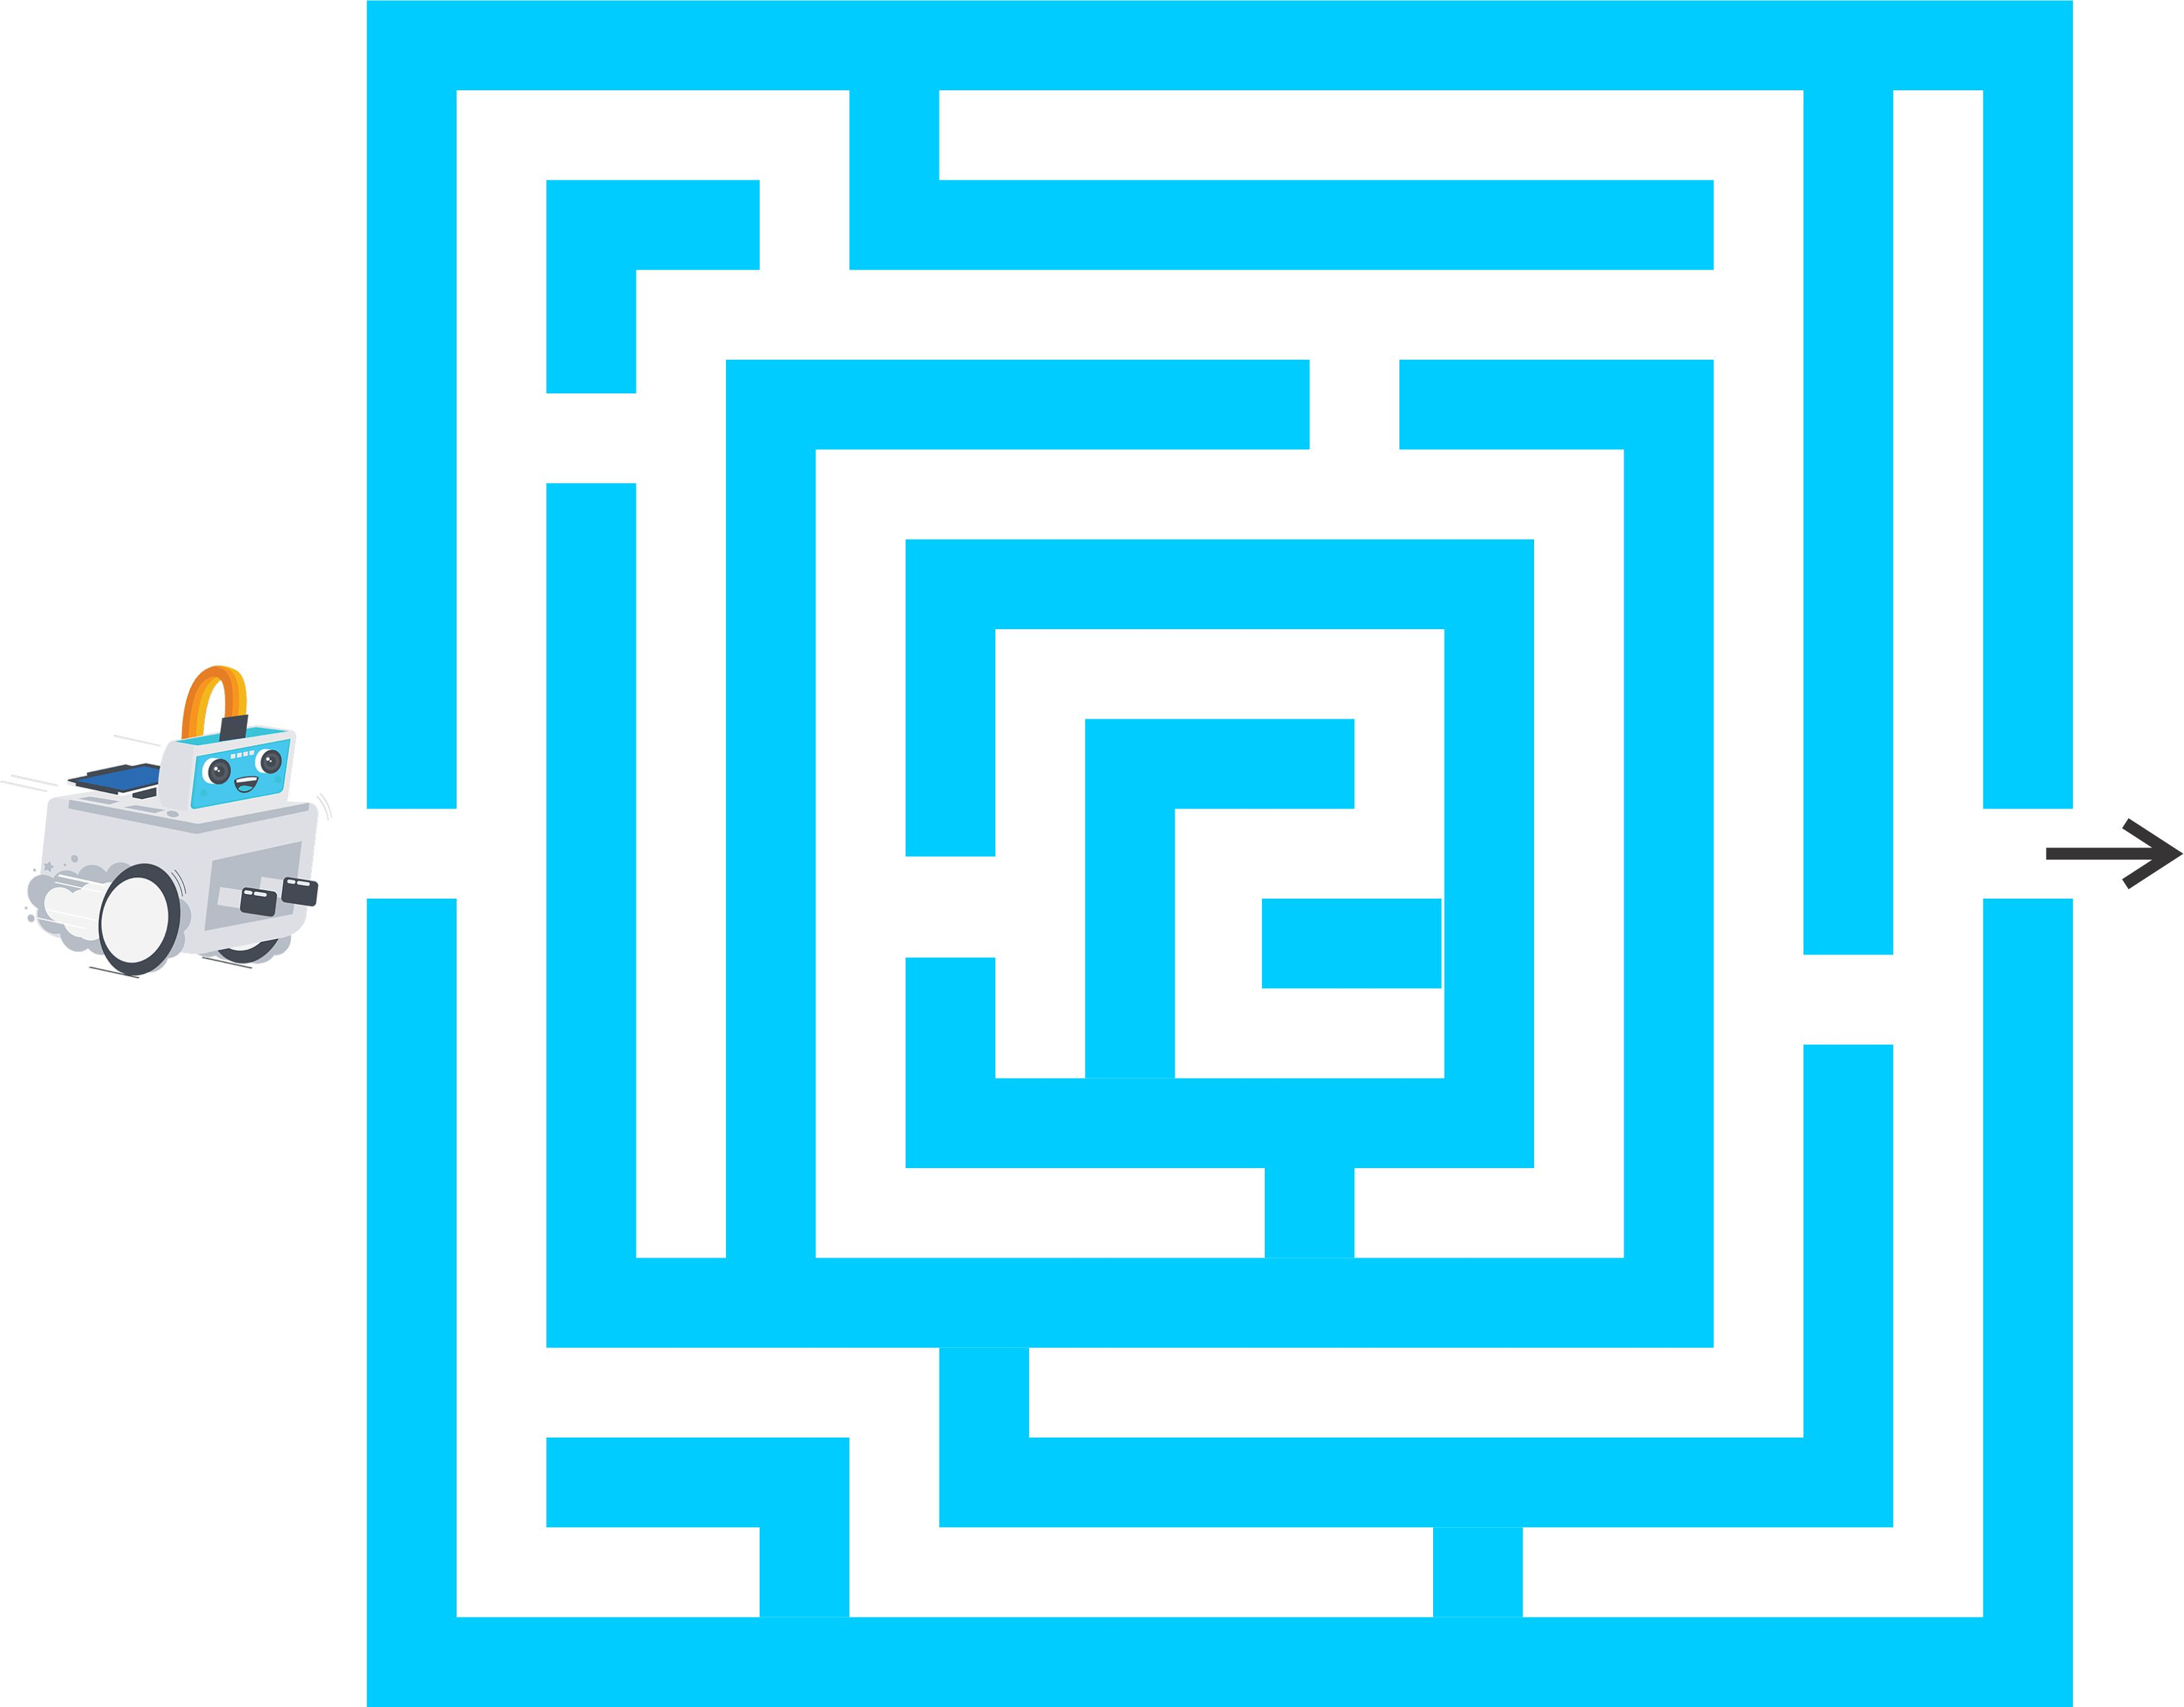
\includegraphics[width=6cm]{Figuras/Labirinto.jpg}
        \label{figura:Labirinto.jpeg}
    \end{figure}
    
 %   \begin{center}
 %       \vspace{6.0cm} 
 %   \end{center}